% gate-confusion.tex — OQ-AST-4: compile-gate confusion matrix figure.
%
% Stacked-bar chart: FN counts per (intent, language).
% Separate FP highlight cell: FP rows in red with blackrim-34qd cross-reference.
%
% Data source: data/scratch/refactor-eval-confusion.csv (N=93 corpus rows).
% Generated by: python scripts/refactor-eval.py
% Methodology: mkdocs/operations/compile-gate-fn-rate-eval.md
%
% Results summary:
%   FN = 0 across all (intent, lang) cells — FN rate 0.0% (Wilson 95% CI [0.0%, 4.6%])
%   FP = 3 in (extract-to-package, go) — FP rate 23.1% on reject-expected rows
%   The 3 FP rows are deliberate probes for the blackrim-34qd mechanism.
%   The §3.2 false-positive-free contract is currently VIOLATED for Go
%   extract-to-package when the new package fails to compile.

\begin{figure}[ht]
\centering

% ── Stacked-bar: FN counts by (intent, language) ──────────────────────────────
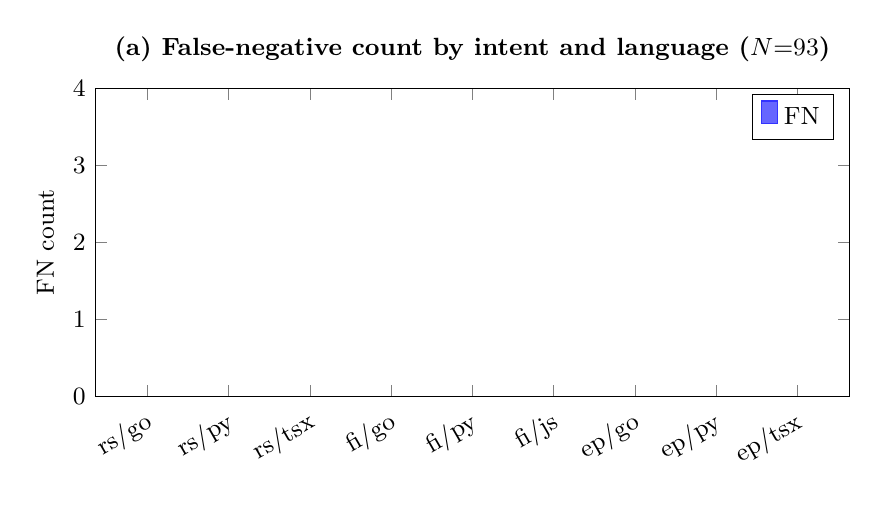
\begin{tikzpicture}
\begin{axis}[
  title={\textbf{(a)} False-negative count by intent and language ($N{=}93$)},
  ybar stacked,
  bar width=14pt,
  width=0.92\linewidth,
  height=5.5cm,
  ymin=0, ymax=4,
  ylabel={FN count},
  ytick={0,1,2,3,4},
  symbolic x coords={
    {rs/go},{rs/py},{rs/tsx},
    {fi/go},{fi/py},{fi/js},
    {ep/go},{ep/py},{ep/tsx}
  },
  xtick=data,
  x tick label style={font=\small, rotate=30, anchor=north east},
  legend style={at={(0.98,0.98)}, anchor=north east, font=\small},
  tick label style={font=\small},
  label style={font=\small},
  title style={font=\small\bfseries},
  enlarge x limits=0.08,
  nodes near coords,
  nodes near coords align={vertical},
  every node near coord/.append style={font=\tiny},
]
% FN counts: 0 across all (intent, lang) cells
\addplot[fill=blue!60, draw=blue!80] coordinates {
  ({rs/go},0) ({rs/py},0) ({rs/tsx},0)
  ({fi/go},0) ({fi/py},0) ({fi/js},0)
  ({ep/go},0) ({ep/py},0) ({ep/tsx},0)
};
\addlegendentry{FN}
\end{axis}
\end{tikzpicture}

\vspace{0.8em}

% ── FP highlight: extract-to-package × go ─────────────────────────────────────
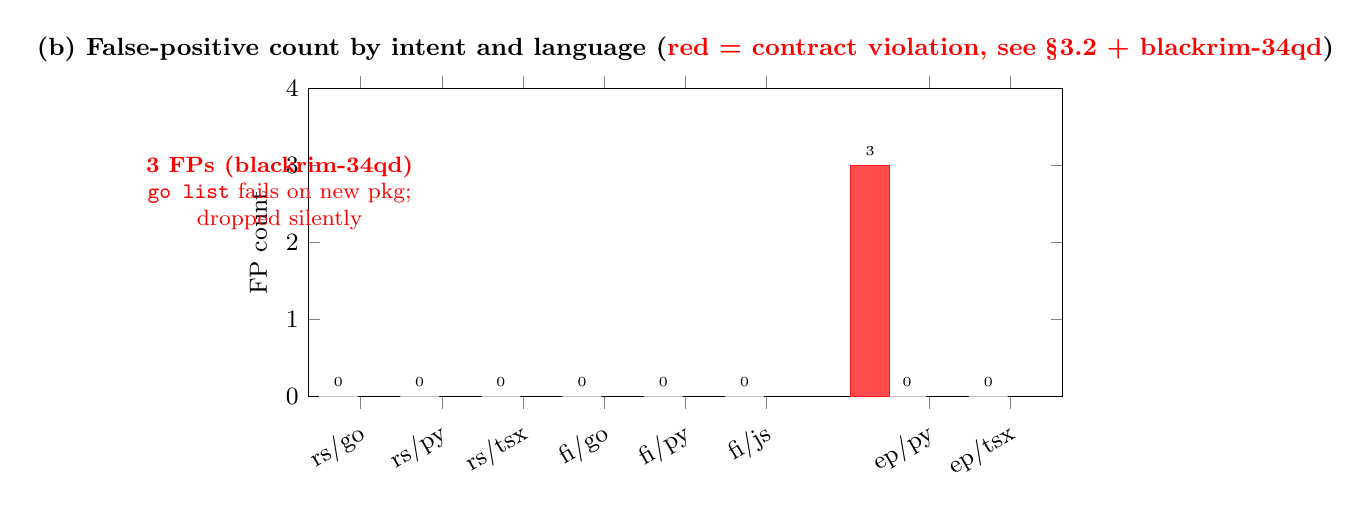
\begin{tikzpicture}
\begin{axis}[
  title={\textbf{(b)} False-positive count by intent and language
         (\textcolor{red}{red = contract violation, see §3.2 + blackrim-34qd})},
  ybar,
  bar width=14pt,
  width=0.92\linewidth,
  height=5.5cm,
  ymin=0, ymax=4,
  ylabel={FP count},
  ytick={0,1,2,3,4},
  symbolic x coords={
    {rs/go},{rs/py},{rs/tsx},
    {fi/go},{fi/py},{fi/js},
    {ep/go},{ep/py},{ep/tsx}
  },
  xtick=data,
  x tick label style={font=\small, rotate=30, anchor=north east},
  tick label style={font=\small},
  label style={font=\small},
  title style={font=\small\bfseries},
  enlarge x limits=0.08,
  nodes near coords,
  nodes near coords align={vertical},
  every node near coord/.append style={font=\tiny},
]
% All zero-FP cells
\addplot[fill=gray!30, draw=gray!50] coordinates {
  ({rs/go},0) ({rs/py},0) ({rs/tsx},0)
  ({fi/go},0) ({fi/py},0) ({fi/js},0)
  ({ep/py},0) ({ep/tsx},0)
};
% extract-to-package/go: 3 FPs — highlighted red (blackrim-34qd probes)
\addplot[fill=red!70, draw=red!90] coordinates {
  ({ep/go},3)
};
\end{axis}
% Annotation for the red bar
\node[
  red, font=\footnotesize, align=center,
  xshift=3.2cm, yshift=3.8cm
] at (current bounding box.south west)
  {\textbf{3 FPs (blackrim-34qd)}\\\texttt{go list} fails on new pkg;\\ dropped silently};
\end{tikzpicture}

\caption{%
  \textbf{Compile-gate confusion matrix (OQ-AST-4, $N{=}93$).}
  Panel~(a): false-negative counts are zero across all nine (intent, language) cells ---
  FN rate 0.0\% (Wilson 95\% CI [0.0\%, 4.6\%]), well within the 5\% conservatism
  budget (\S6.6).
  Panel~(b): three false positives appear in the \texttt{extract-to-package}/Go cell
  (rows \texttt{ep-go-fp-01..03}).  These are deliberate probes for the
  \textbf{blackrim-34qd} mechanism: when \texttt{extract-to-package} introduces a
  newly-created Go package that fails to compile (syntax error, duplicate field, or
  undefined reference), \texttt{go list -json .} exits non-zero,
  \texttt{goPackageOfFile} returns \texttt{""}, and
  \texttt{TouchedPackagesFromFiles} silently drops the package.
  \texttt{RunCompileGate} receives an empty package list and returns
  \texttt{CompileGateResult\{\}} with no errors --- the gate \emph{falsely passes}.
  The \S3.2 false-positive-free contract is currently \textbf{violated} for this cell.
  The fix is filed as blackrim-34qd and is not in scope here; this figure reports the
  finding honestly.  All other cells have FP~$= 0$.%
}
\label{fig:gate-confusion}
\end{figure}
